\section{Algoritmos envolvendo polígonos}

\begin{frame}[fragile]{Perímetro}

    \begin{itemize}
        \item O perímetro de um polígono consiste na medida de seu contorno, isto é, a soma dos 
            comprimentos de suas aresta
        \pause

        \item Ele pode ser calculado diretamente a partir da representação do polígono por meio
            de seus vértices
        \pause
    \end{itemize}

    \inputsnippet{cpp}{43}{56}{codes/polygon.cpp}
\end{frame}

\begin{frame}[fragile]{Área}

    \begin{itemize}
        \item A área delimitada por um polígono pode ser também determinada diretamente a partir
            de seus vértices
        \pause

        \item Ela corresponde à metade do valor absoluto do \lq \lq determinante\rq\rq\ abaixo (as 
            aspas significam que a notação remete a um determinante, mas não é um determinante de 
                fato, uma vez que a matriz não é quadrada)
        \begin{align*}
            A &= \frac{1}{2}\begin{vmatrix}
                x_0 & y_0 \\
                x_1 & y_1 \\
                x_2 & y_2 \\
                \ldots & \ldots \\
                x_{n-1} & y_{n-1} \\
            \end{vmatrix} \\
            & = \frac{1}{2}|x_0y_1 + x_1y_2 + \ldots + x_{n-1}y_0 - x_1y_0 - x_2y_1 - \ldots - x_0y_{n-1}|
        \end{align*}
    \end{itemize}

\end{frame}

\begin{frame}[fragile]{Implementação da área do polígono}
    \inputsnippet{cpp}{58}{69}{codes/polygon.cpp}
\end{frame}

\begin{frame}[fragile]{Área de polígonos regulares}

    \begin{itemize}
        \item Um polígono é dito regular se todos os seus lados têm a mesma medida
        \pause

        \item A área também pode ser computada através do conhecimento do número de lados $n$ e um 
            dos três valores abaixo:
        \pause
            \begin{enumerate}
                \item o comprimento de um dos lados ($s$)
        \pause
                \item a apótema, isto é, o raio do círculo inscrito ($r$)
        \pause
                \item o raio do círculo circunscrito ($R$)
            \end{enumerate}
        \pause

        \item As expressões abaixo relacionam a área do polígono regular com as medidas
            supracitadas:
        \[
            A = \frac{1}{2}nrs = \frac{1}{4}ns^2\cot \frac{\pi}{n} = nr^2\tan \frac{\pi}{n} = \frac{1}{2}nR^2\sin \frac{2\pi}{n}
        \]

    \end{itemize}

\end{frame}

\begin{frame}[fragile]{Relação entre pontos e polígonos}

    \begin{itemize}
        \item Para se verificar se um ponto $P$ está localizado, ou não, no interior de um 
            polígono, basta computar a soma dos ângulos formados por $P$ e cada par de vértices do 
            polígono
        \pause

        \item Esta soma deve adicionar o ângulo se o ponto está na mesma orientação do polígono, e
        subtrair em caso contrário
        \pause

        \item Se o total for igual a $2\pi$, o ponto está no interior do polígono
        \pause

        \item Esta verificação vale tanto para polígonos convexos quanto côncavos

    \end{itemize}

\end{frame}

\begin{frame}[fragile]{Implementação da relação entre pontos e polígonos}
    \inputsnippet{cpp}{72}{88}{codes/polygon.cpp}
\end{frame}

\begin{frame}[fragile]{Implementação da relação entre pontos e polígonos}
    \inputsnippet{cpp}{90}{109}{codes/polygon.cpp}
\end{frame}

\begin{frame}[fragile]{Relação entre polígonos e retas}

    \begin{itemize}
        \item Considere uma reta $r$, que passa pelos pontos $A$ e $B$, e um polígono convexo $P$, 
            com $n$ vértices
        \pause

        \item A reta $r$ secciona o polígono em duas regiões, esquerda e direita, que podem ser ou 
            uma vazia e outra contendo $P$ integralmente, ou serem compostas de dois polígonos 
            convexos $P_1$ e $P_2$, resultantes do corte de $P$ por $r$
        \pause

        \item A rotina \code{cpp}{cut_polygon()}, apresentada a seguir e adaptada de Competitive 
            Programming 3, retorna a região a esquerda do corte, considerando que $P$ está descrito 
            no sentido anti-horário
    \end{itemize}
        \pause

    \begin{figure}
        \centering

        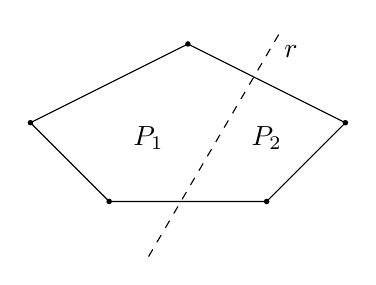
\begin{tikzpicture}
            \coordinate (A) at (1, 1);
            \coordinate (B) at (3, 1);
            \coordinate (C) at (4, 2);
            \coordinate (D) at (2, 3);
            \coordinate (E) at (0, 2);

            \draw (A) -- (B) -- (C) -- (D) -- (E) -- (A);

            \draw[dashed] (1.5, 0.3) -- (3.2, 3.2);
            \node[anchor=west] at (3.1, 2.9) { $r$ };
            \node at (3, 1.8) { $P_2$ };
            \node at (1.5, 1.8) { $P_1$ };

            \fill (A) circle [radius=1pt];
            \fill (B) circle [radius=1pt];
            \fill (C) circle [radius=1pt];
            \fill (D) circle [radius=1pt];
            \fill (E) circle [radius=1pt];

        \end{tikzpicture}
    \end{figure}

\end{frame}

\begin{frame}[fragile]{Implementação da relação entre pontos e retas}
    \inputsnippet{cpp}{112}{131}{codes/polygon.cpp}
\end{frame}

\begin{frame}[fragile]{Implementação da relação entre pontos e retas}
    \inputsnippet{cpp}{132}{148}{codes/polygon.cpp}
\end{frame}

\begin{frame}[fragile]{Círculo circunscrito}

    \begin{itemize}
        \item Um polígono regular (medidas dos lados iguais) de $n$ lados possui um círculo 
            circunscrito (cujos vértices pertencem ao círculo) e um círculo inscrito 
            (cujos lados são tangentes ao círculo)
        \pause

        \item O raio $R$ do círculo circunscrito é igual ao raio do polígono: a distância entre o 
            seu centro e um de seus vértices
        \pause

        \item Se $s$ é a medida do lado do polígono, então
        \[
            \sin \frac{\pi}{n} = \frac{(s/2)}{R},
        \]
        isto é,
        \[
            R = \frac{s}{2}\csc\frac{\pi}{n}
        \]

    \end{itemize}

\end{frame}

\begin{frame}[fragile]{Visualização do círculo circunscrito}

    \def\R{3}

    \begin{figure}
        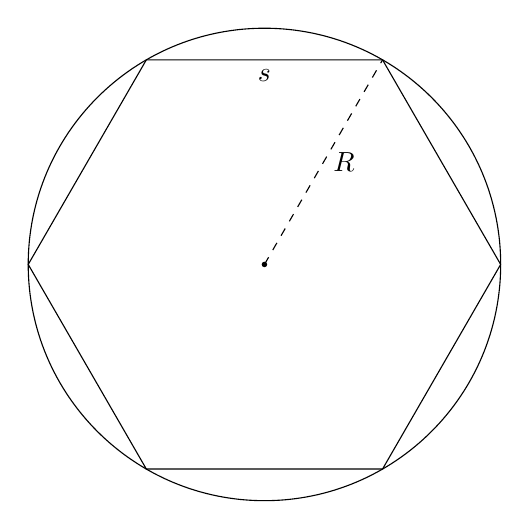
\begin{tikzpicture}
            \draw (0:\R) -- (60:\R) -- node[anchor=north] { $s$ } (120:\R) -- (180:\R) -- (240:\R) -- (300:\R) -- (360:\R) -- (0:\R);
            \draw (0, 0) circle [radius=\R];
            \fill (0, 0) circle [radius=1pt];
            \draw[dashed] (0, 0) -- node[anchor=west] { $R$ } (60:\R);

        \end{tikzpicture}
    \end{figure}

\end{frame}

\begin{frame}[fragile]{Implementação do cálculo do raio $R$ do círculo circunscrito}
    \inputsnippet{cpp}{150}{156}{codes/polygon.cpp}
\end{frame}

\begin{frame}[fragile]{Círculo inscrito}

    \begin{itemize}
        \item O raio $r$ do círculo inscrito pode ser determinado a partir da medida 
            $s$ de um dos lados do polígono regular, através da relação
        \[
            \tan \frac{\pi}{n} = \frac{(s/2)}{r},
        \]
        isto é,
        \[
            r = \frac{s}{2}\cot\frac{\pi}{n}
        \]
        \pause

        \item O raio $r$ também é denominado apótema do polígono regular
        \pause

        \item Os raios $R$ e $r$ se relacionam de modo que
        \[
            r = R\cos \frac{\pi}{n}
        \]
    \end{itemize}

\end{frame}

\begin{frame}[fragile]{Visualização do círculo inscrito}

    \def\R{3}

    \begin{figure}
        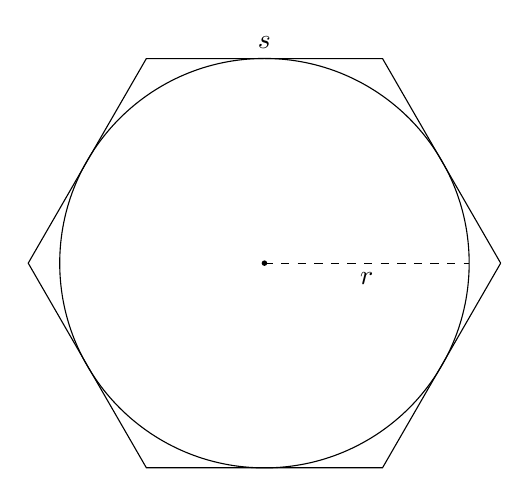
\begin{tikzpicture}
            \draw (0:\R) -- (60:\R) -- node[anchor=south] { $s$ } (120:\R) -- (180:\R) -- (240:\R) -- (300:\R) -- (360:\R) -- (0:\R);
            \draw (0, 0) circle [radius=2.6];
            \fill (0, 0) circle [radius=1pt];
            \draw[dashed] (0, 0) -- node[anchor=north] { $r$ } (2.6, 0);

        \end{tikzpicture}
    \end{figure}

\end{frame}

\begin{frame}[fragile]{Implementação do cálculo do raio $r$ do círculo inscrito}
    \inputsnippet{cpp}{158}{164}{codes/polygon.cpp}
\end{frame}


